

\chapter{Functions}\label{chapter:functions}
\begin{center}
\begin{tabular}[h]{lccc}
   Function to scalar
   & $f : \mathbb R^n \to \mathbb R$
   & $f(x) \in \mathbb R$
   & $\{f \leftarrow x\}$
   \\
   Function to vector
   & $g : \mathbb R^n \to \mathbb R^m$
   & $g(x) \in \mathbb R^m$
   & 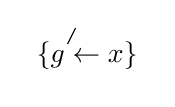
\begin{tikzpicture}[baseline=-.25em]
      \node (0,0) {$\{g \leftarrow x\}$};
      \draw (-.25, .15) -- ++(.1,.2);
   \end{tikzpicture}
   \\
   Element-wise function
   & $h : \mathbb R^n \to \mathbb R$
   & $h(x) \in \mathbb R^m$
   & 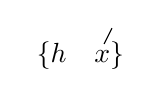
\begin{tikzpicture}[baseline=-.25em]
      \node (0,0) {$\{h \quad x\}$};
      \draw (.3, .15) -- ++(.1,.2);
   \end{tikzpicture}
   \\
   Vector times vector function
   & $u : \mathbb R^n \to \mathbb R^m, v \in \mathbb R^m$
   & $v^T u(x) \in \mathbb R$
   & \begin{tikzpicture}[baseline=-.25em]
      \node (v) at (0,0) {$v$};
      \node (u) at (1,0) {$\{u \leftarrow x\}$};
      \path (v) edge [out=140, in=40, looseness=1] ($(u.west) + (1.5em,.5em)$);
   \end{tikzpicture}
   \\
   Vector times matrix function
   & $A : \mathbb R^n \to \mathbb R^{m\times n}, v \in \mathbb R^n$
   & $A(x)v \in \mathbb R^m$
   & 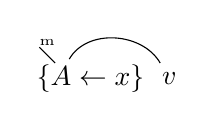
\begin{tikzpicture}[baseline=-.25em]
      \node (A) at (0,0) {$\{A \leftarrow x\}$};
      \node (x) at (1,0) {$v$};
      \draw (-.27, .25) edge[out=60, in=120, looseness=1] (x);
      \draw (-.45, .2) -- ++(-.2,.2) node[midway, above, font=\tiny] {m};
   \end{tikzpicture}
   \\
   Batch function application
   & $f : \mathbb R^d \to \mathbb R, X \in \mathbb R^{b\times d}$
   & $f(X) \in \mathbb R^b$
   & \begin{tikzpicture}[baseline=-.25em]
      \node (f) at (0,0) {$\{f \leftarrow X\}$};
      \draw ($(f.east) + (-.35, .25)$) --  ++(.1,.2) node[midway, above, font=\tiny] {b};
   \end{tikzpicture}
\end{tabular}
\end{center}

As an example of a more complicated function, let $\exp : \mathbb R \to \mathbb R$ be the element-wise exponential function,
and $\mathrm{pow}^{-1} : \mathbb R \to \mathbb R$ be the element-wise inverse power function.
Then we can write $\mathrm{softmax}:\mathbb R^d \to \mathbb R^d$ as the tensor diagram:
\[
   \mathrm{softmax}(x) =
   \begin{tikzpicture}[baseline=-.25em]
      \node (ex) at (0,0) {$\{\mathrm{exp} \quad x\}$};
      \node[right=1em of ex] (p) {$\{\mathrm{pow}^{-1} \quad \{\mathrm{exp} \quad x\}\quad \sbullet\,\}$};
      \draw ($(p.east)+(-1.1,.15)$) edge[out=90, in=90, looseness=1] ($(p.east)+(-.4,.15)$);
      \draw ($(ex) + (.5, .15)$) -- ++(.1,.2);
   \end{tikzpicture}
   .
\]
Note in particular how
\begin{tikzpicture}[baseline=-.25em]
   \node (p) {$\{\mathrm{exp} \quad x\}\quad \sbullet$};
   \path ($(p.east)+(-.9,.15)$) edge [out=90, in=90, looseness=1] ($(p.east)+(-.2,.15)$);
\end{tikzpicture}
is the diagram way of writing $\sum_i \exp(x_i)$.
Alternatively we could have used a function $\mathrm{sum} : \mathbb R^n \to \mathbb R$, but the more we can express in terms of tensor diagrams, the more we can use the powerful tensor diagram calculus.



Stuff about analytical matrix functions.
Such as Exponential Matrix Function.
I'd rather talk about my general function notation.
And maybe about taylor series?


\newpage
\section{The Chain Rule}
Sometimes the objective is to find the derivative of a matrix which is a function of another matrix.

E.g. $f : \R^n -> \R^n$

Standard chain rule.
Here we let $f\in\mathbb R^d\to \mathbb R$ be a scalar function, and $v\in\mathbb R^d\to \mathbb R^d$ be a vector function as used in backprop.

Visualization of the Chain Rule: $J_{f\circ v}(x) = \nabla_{\!f}(v(x)) J_v(x)$.

\[
   \begin{tikzpicture}[baseline=-.25em, inner sep=1pt]
      \node (n1) {$(\quad\{$};
      \node[right=.5em of n1] (n2) {$f$};
      \node[right=.5em of n2] (n3) {$\{$};
      \node[right=0em of n3] (n4) {$v$};
      \node[right=1em of n4] (n5) {$x$};
      \node[right=0em of n5] (n6) {$\}\}\quad)$};
      \draw (n4) edge[out=90, in=90, looseness=1, ->] (n2);
      \draw (n5) edge[->] (n4);
      \draw[d] (n6.east) -- ++(.2,.2);
   \end{tikzpicture}
   =
   \begin{tikzpicture}[baseline=-.25em, inner sep=1pt]
      \node (n1) {$\{$};
      \node[right=.5em of n1] (n2) {$f$};
      \node[right=.5em of n2] (n3) {$\{$};
      \node[right=0em of n3] (n4) {$v$};
      \node[right=1em of n4] (n5) {$x$};
      \node[right=0em of n5] (n6) {$\}\}$};
      \node[right=1em of n6] (n7) {$\{$};
      \node[right=0em of n7] (n8) {$v$};
      \node[right=1em of n8] (n9) {$x$};
      \node[right=0em of n9] (n10) {$\}$};
      \draw (n4) edge[out=90, in=90, looseness=1, ->] (n2);
      \draw (n5) edge[->] (n4);
      \draw (n9) edge[->] (n8);
      \draw[d1] (n2) edge[out=-30, in=-120, looseness=1] (n8);
      \draw[d1] (n8) -- ++(.3,.3);
   \end{tikzpicture}
\]

\subsection{The Chain Rule}
Let $f\in\mathbb R^d\to \mathbb R$ be a scalar function, and $v\in\mathbb R^d\to \mathbb R^d$ be a vector function, as used in backprop.
Then we can write the chain rule as:
\[
   \begin{tikzpicture}[baseline=-1em, inner sep=1pt]
      \node (n0) {$f$};
      \node[below=1em of n0] (n1) {$v$};
      \node[below=1em of n1] (n2) {$x$};
      \draw[->] (n2) -- (n1);
      \draw[->] (n1) -- (n0);
      \drawellipse{0}{-.55}{.5}{1}{180/4}
   \end{tikzpicture}
   =
   \hspace{.5em}
   \begin{tikzpicture}[baseline=-1em, inner sep=1pt]
      \node[dn] (n0) {$f$};
      \node[below=1em of n0] (n1) {$v$};
      \node[below=1em of n1] (n2) {$x$};
      \node[right=1em of n0, dn] (n3) {$v$};
      \node[below=1em of n3] (n4) {$x$};
      \draw[->] (n2) -- (n1);
      \draw[->] (n1) -- (n0);
      \draw[->] (n4) -- (n3);
      \draw[d0] (n0) -- (n3);
      \draw[d0] (n3) -- ++(.5,0);
   \end{tikzpicture}
\]
Using standard notation:
$J_{f\circ v}(x) = \nabla_{\!f}(v(x)) J_v(x)$.

\vspace{1em}

The second derivative, (or Hessian Chain rule):
\[
   \begin{tikzpicture}[baseline=-1em, inner sep=1pt]
      \node (n0) {$f$};
      \node[below=1em of n0] (n1) {$v$};
      \node[below=1em of n1] (n2) {$x$};
      \draw[->] (n2) -- (n1);
      \draw[->] (n1) -- (n0);
      \drawellipse{0}{-.55}{.5}{1}{180/4}
      \drawellipse{0}{-.55}{.7}{1.2}{180/4}
   \end{tikzpicture}
   =
   \hspace{.5em}
   \begin{tikzpicture}[baseline=-1em, inner sep=1pt]
      \node[dn] (n0) {$f$};
      \node[below=1em of n0] (n1) {$v$};
      \node[below=1em of n1] (n2) {$x$};
      \node[right=1em of n0, dn] (n3) {$v$};
      \node[below=1em of n3] (n4) {$x$};
      \draw[->] (n2) -- (n1);
      \draw[->] (n1) -- (n0);
      \draw[->] (n4) -- (n3);
      \draw[d0] (n0) -- (n3);
      \draw[d0] (n3) -- ++(.5,0);
      \drawellipse{.4}{-.55}{1}{1.2}{180/4}
   \end{tikzpicture}
   =
   \hspace{.5em}
   \begin{tikzpicture}[baseline=-1em, inner sep=1pt]
      \node[dn] (n0) {$f$};
      \node[below=1em of n0] (n1) {$v$};
      \node[below=1em of n1] (n2) {$x$};
      \node[right=1.5em of n0, dn] (n3) {$v$};
      \node[below=1em of n3] (n4) {$x$};
      \draw[->] (n2) -- (n1);
      \draw[->] (n1) -- (n0);
      \draw[->] (n4) -- (n3);
      \draw[d0] (n0) -- (n3);
      \draw[d0] (n3) -- ++(.5,0);
      \drawellipse{0}{-.55}{.5}{1.2}{180/4}
   \end{tikzpicture}
   +
   \hspace{.5em}
   \begin{tikzpicture}[baseline=-1em, inner sep=1pt]
      \node[dn] (n0) {$f$};
      \node[below=1em of n0] (n1) {$v$};
      \node[below=1em of n1] (n2) {$x$};
      \node[right=1.5em of n0, dn] (n3) {$v$};
      \node[below=1em of n3] (n4) {$x$};
      \draw[->] (n2) -- (n1);
      \draw[->] (n1) -- (n0);
      \draw[->] (n4) -- (n3);
      \draw[d0] (n0) -- (n3);
      \draw[d0] (n3) -- ++(.5,0);
      \drawellipse{1}{-.25}{.5}{.7}{180/4}
   \end{tikzpicture}
   =
   \hspace{.5em}
   \begin{tikzpicture}[baseline=-1em, inner sep=1pt]
      \node[ddn] (n0) {$f$};
      \node[below=1em of n0] (n1) {$v$};
      \node[below=1em of n1] (n2) {$x$};
      \node[right=1em of n0, yshift=-1em, dn] (n3) {$v$};
      \node[below=1em of n3] (n4) {$x$};
      \node[right=1.5em of n3, yshift=1em, dn] (n5) {$v$};
      \node[below=1em of n5] (n6) {$x$};
      \draw[->] (n2) -- (n1);
      \draw[->] (n1) -- (n0);
      \draw[->] (n4) -- (n3);
      \draw[->] (n6) -- (n5);
      \draw[d0] (n0) -- (n3);
      \draw[d0] (n0) -- (n5);
      \draw[d0] (n3) -- ++(.5,0);
      \draw[d0] (n5) -- ++(.5,0);
   \end{tikzpicture}
   +
   \hspace{.5em}
   \begin{tikzpicture}[baseline=-1em, inner sep=1pt]
      \node[dn] (n0) {$f$};
      \node[below=1em of n0] (n1) {$v$};
      \node[below=1em of n1] (n2) {$x$};
      \node[right=1.5em of n0, ddn] (n3) {$v$};
      \node[below=1em of n3] (n4) {$x$};
      \draw[->] (n2) -- (n1);
      \draw[->] (n1) -- (n0);
      \draw[->] (n4) -- (n3);
      \draw[d0] (n0) -- (n3);
      \draw[d0] (n3) -- ++(.5,0);
      \draw[d0] ($(n3)+(.166,.15)$) -- ++(.4,0);
   \end{tikzpicture}
\]
Using standard notation:
\(
H_{f\circ v}(x) = Dv(x)^T \cdot D^2f(v(x)) \cdot Dv(x) + \sum_{k=1}^d \frac{\partial f}{\partial u_k}(v(x)) \frac{\partial^2 v_k}{\partial x \partial x^T}(x).
\)


\begin{align*}
\hspace{-2em}
   \frac{\partial A(x)x}{\partial x}
   &= (x^T \otimes I) \frac{\partial}{\partial x}  \mathrm{vec}[A(x)] + A(x)
   &
   \begin{tikzpicture}[baseline=-.25em, inner sep=1pt]
      \node (n0) at (0,0) {$($};
      \node[right=.5em of n0] (x0) {$x$};
      \node[right=.5em of x0] (n2) {$\{$};
      \node[right=.5em of n2] (A) {$A$};
      \node[right=1em of A] (x1) {$x$};
      \node[right=.5em of x1] (n5) {$\})$};
      \draw[->] (x1) -- (A);
      \draw (x0) edge[out=90, in=90, looseness=1] (A);
      \draw[d] (n5.east) -- ++(.2,.2);
   \end{tikzpicture}
   &=
   \begin{tikzpicture}[baseline=-.25em, inner sep=1pt]
      \node (x0) {$x$};
      \node [right=.5em of x0] (n2) {$(\{$};
      \node [right=.5em of n2] (A) {$A$};
      \node [right=1em of A] (x1) {$x$};
      \node [right=.5em of x1] (n5) {$\})$};
      \draw[->] (x1) -- (A);
      \draw (x0) edge[out=90, in=90, looseness=1] (A);
      \draw[d] (n5.east) -- ++(.2,.2);
   \end{tikzpicture}
 +
   \begin{tikzpicture}[baseline=-.25em, inner sep=1pt]
      \node (n0) at (0,0) {$($};
      \node [right=.5em of n0] (x0) {$x$};
      \node [right=.5em of x0] (n1) {$)$};
      \node [right=.5em of n1] (n2) {$\{$};
      \node [right=.5em of n2] (A) {$A$};
      \node [right=1em of A] (x1) {$x$};
      \node [right=.5em of x1] (n5) {$\}$};
      \draw[->] (x1) -- (A);
      \draw (x0) edge[out=90, in=90, looseness=1] (A);
      \draw[d] (n1.east) -- ++(.2,.2);
   \end{tikzpicture}
 \\&&&=
   \begin{tikzpicture}[baseline=-.25em, inner sep=1pt]
      \node (x0) {$x$};
      \node [right=.5em of x0] (n2) {$\{$};
      \node [right=.5em of n2] (A) {$A$};
      \node [right=1em of A] (x1) {$x$};
      \node [right=.5em of x1] (n5) {$\}$};
      \draw[->] (x1) -- (A);
      \draw (x0) edge[out=90, in=90, looseness=1] (A);
      \draw[d] ($(A.east)+(.1,.1)$) -- ++(.3,.2);
   \end{tikzpicture}
 +
   \begin{tikzpicture}[baseline=-.25em, inner sep=1pt]
      \node (n2) {$\{$};
      \node [right=.5em of n2] (A) {$A$};
      \node [right=1em of A] (x1) {$x$};
      \node [right=.5em of x1] (n5) {$\}$};
      \draw[->] (x1) -- (A);
      \draw (A) -- ++(.4,.3);
   \end{tikzpicture}
\end{align*}

\[
   \begin{tikzpicture}[baseline=-1em, inner sep=1pt]
      \node (n0) {$A$};
      \node[below=1em of n0] (n1) {$x$};
      \node[right=1em of n0] (n2) {$x$};
      \draw[->] (n1) -- (n0);
      \draw (n2) -- (n0);
      \drawellipse{.25}{-.25}{.7}{.7}{180/4}
      \draw (n0) -- ++(-.5,0);
   \end{tikzpicture}
   =
   \hspace{.5em}
   \begin{tikzpicture}[baseline=-1em, inner sep=1pt]
      \node (n0) {$A$};
      \node[below=1em of n0] (n1) {$x$};
      \node[right=1em of n0] (n3) {$x$};
      \draw[->] (n1) -- (n0);
      \draw (n0) -- (n3);
      \drawellipse{0}{-.25}{.4}{.7}{180/4}
      \draw (n0) -- ++(-.5,0);
   \end{tikzpicture}
   +
   \hspace{.5em}
   \begin{tikzpicture}[baseline=-1em, inner sep=1pt]
      \node (n0) {$A$};
      \node[below=1em of n0] (n1) {$x$};
      \node[right=.75em of n0] (n3) {$x$};
      \draw[->] (n1) -- (n0);
      \draw (n0) -- (n3);
      \draw (n0) -- ++(-.5,0);
      \drawellipse{.575}{0}{.25}{.25}{180/4}
   \end{tikzpicture}
   =
   \hspace{.5em}
   \begin{tikzpicture}[baseline=-1em, inner sep=1pt]
      \node[dn] (n0) {$A$};
      \node[below=1em of n0] (n1) {$x$};
      \node[right=.75em of n0] (n3) {$x$};
      \draw[->] (n1) -- (n0);
      \draw (n0) -- (n3);
      \draw[d0] (n0) -- ++(.4,.4);
      \draw (n0) -- ++(-.5,0);
   \end{tikzpicture}
   +
   \hspace{.5em}
   \begin{tikzpicture}[baseline=-1em, inner sep=1pt]
      \node (n0) {$A$};
      \node[below=1em of n0] (n1) {$x$};
      \draw[->] (n1) -- (n0);
      \draw (n0) -- ++(.5,0);
      \draw (n0) -- ++(-.5,0);
   \end{tikzpicture}
\]


are common. All pixel-adaptive filters like non-local means, bilateral, etc, and the so-called attention mechanism in transformers can be written this way

Gradient of this f(x) is important \& has a form worth remembering…


\subsubsection{Trace identity}
Assume F(X) to be a differentiable function of each of the elements of X. It
then holds that
\[\frac{d \mathrm{Tr}(F(x))}{dX} = f(X)^T,\]
where $f(\cdot)$ is the scalar derivative of $F(\cdot)$.

TODO: To show this with tensor diagrams, we first need to introduce our notation for functions.

For example
$$
\frac{\partial \operatorname{Tr}(\sin (\mathbf{X}))}{\partial \mathbf{X}}=\cos (\mathbf{X})^T
$$
% Many more examples here: https://mbustamanter.github.io/ssg-blog/matder1/


\subsubsection{Pseudo-linear form}
Maybe this should just be an example in a table?

Derivation of Peyman Milanfar's gradient
\begin{align*}
\mathrm{d}[\mathbf{f}(\mathbf{x})] & =\mathrm{d}[\mathbf{A}(\mathbf{x}) \mathbf{x}] \\
& =\mathrm{d}[\mathbf{A}(\mathbf{x})] \mathbf{x}+\mathbf{A}(\mathbf{x}) \mathrm{d} \mathbf{x} \\
& =\operatorname{vec}\{\mathrm{d}[\mathbf{A}(\mathbf{x})] \mathbf{x}\}+\mathbf{A}(\mathbf{x}) \mathrm{d} \mathbf{x} \\
& =\operatorname{vec}\{\mathbf{I} \mathrm{d}[\mathbf{A}(\mathbf{x})] \mathbf{x}\}+\mathbf{A}(\mathbf{x}) \mathrm{d} \mathbf{x} \\
& =\left(\mathbf{x}^T \otimes \mathbf{I}\right) \operatorname{vec}\{\mathrm{d}[\mathbf{A}(\mathbf{x})]\}+\mathbf{A}(\mathbf{x}) \mathrm{d} \mathbf{x} \\
& =\left(\mathbf{x}^T \otimes \mathbf{I}\right) \mathrm{D} \operatorname{vec}[\mathbf{A}(\mathbf{x})] \mathrm{d} \mathbf{x}+\mathbf{A}(\mathbf{x}) \mathrm{d} \mathbf{x} \\
& =\left[\left(\mathbf{x}^T \otimes \mathbf{I}\right) \mathrm{D} \operatorname{vec}[\mathbf{A}(\mathbf{x})]+\mathbf{A}(\mathbf{x})\right] \mathrm{d} \mathbf{x}
\end{align*}

\subsection{Taylor}
For an n-times differentiable function $v: \R^d\to\R^d$ we can write the Taylor expansion:
\begin{align*}
    v(x + \eps)
    &\approx
    v(x)
    + \left[\frac{\partial}{\partial x} v(x)\right]\eps
    + \frac{1}{2}\left[\frac{\partial}{\partial x}\left[\frac{\partial}{\partial x} v(x)\right]\eps\right]\eps
    + \frac{1}{6}\left[\frac{\partial}{\partial x}\left[\frac{\partial}{\partial x} \left[\frac{\partial}{\partial x} v(x)\right]\eps\right]\eps\right]\eps
    + \dots
    \\
    &=
    v(x)
    + \left[\frac{\partial}{\partial x} v(x)\right]\eps
    +
    \frac{1}{2}
    (I \otimes \eps)
    \left[\frac{\partial\mathrm{vec}}{\partial x}\left[\frac{\partial v(x)}{\partial x} \right]\right]\eps
    + \frac{1}{6}
    (I \otimes \eps \otimes \eps)
    \left[\frac{\partial\mathrm{vec}}{\partial x}\left[\frac{\partial\mathrm{vec}}{\partial x} \left[\frac{\partial v(x)}{\partial x} \right]\right]\right]\eps
    + \dots
\end{align*}
Or with indices:
\begin{align*}
    v_i(x + \eps)
    &\approx
    v_i(x)
    + \sum_j \frac{\partial v_i(x)}{\partial x_j} \eps_j
    + \frac12 \sum_{j,k} \frac{\partial v_i(x)}{\partial x_j\partial x_k} \eps_j \eps_k
    + \frac16 \sum_{j,k,\ell} \frac{\partial v_i(x)}{\partial x_j\partial x_k\partial x_\ell} \eps_j \eps_k \eps_\ell
\end{align*}
Or diagrams:
\[
   \begin{tikzpicture}[baseline=-1em, inner sep=1pt]
      \node (n0) {$v$};
      \node[below=1em of n0] (n1) {$(x+\eps)$};
      \draw[->] (n1) -- (n0);
      \draw (n0) -- ++(.5,0);
   \end{tikzpicture}
   \approx
   \begin{tikzpicture}[baseline=-1em, inner sep=1pt]
      \node (n0) {$v$};
      \node[below=1em of n0] (n1) {$x$};
      \draw[->] (n1) -- (n0);
      \draw (n0) -- ++(.5,0);
   \end{tikzpicture}
   +
   \begin{tikzpicture}[baseline=-1em, inner sep=1pt]
      \node[dn] (n0) {$v$};
      \node[below=1em of n0] (n1) {$x$};
      \node[left=1em of n0] (n2) {$\eps$};
      \draw[->] (n1) -- (n0);
      \draw[d0] (n0) -- (n2);
      \draw (n0) -- ++(.5,0);
   \end{tikzpicture}
   +\frac12
   %\hspace{.5em}
   \begin{tikzpicture}[baseline=-1em, inner sep=1pt]
      \node[ddn] (n0) {$v$};
      \node[below=1em of n0] (n1) {$x$};
      \node[left=1em of n0] (n2) {$\eps$};
      \node[left=.75em of n0, yshift=-1em] (n3) {$\eps$};
      \draw[->] (n1) -- (n0);
      \draw[d0] (n0) -- (n2);
      \draw[d0] (n0) -- (n3);
      \draw (n0) -- ++(.5,0);
   \end{tikzpicture}
   +
   \frac16
   %\hspace{.5em}
   \begin{tikzpicture}[baseline=-1em, inner sep=1pt]
      \node[dddn] (n0) {$v$};
      \node[below=1em of n0] (n1) {$x$};
      \node[left=1em of n0] (n2) {$\eps$};
      \node[left=.75em of n0, yshift=-1em] (n3) {$\eps$};
      \node[left=.75em of n0, yshift=1em] (n4) {$\eps$};
      \draw[->] (n1) -- (n0);
      \draw[d0] (n0) -- (n2);
      \draw[d0] (n0) -- (n3);
      \draw[d0] (n0) -- (n4);
      \draw (n0) -- ++(.5,0);
   \end{tikzpicture}
   +
   \dots
\]

TODO: Examples based on idempotent matrices etc.



